\renewcommand{\prevlecture}{0}
\renewcommand{\thislecture}{0}
\renewcommand{\nextlecture}{1}

%
% Cover page
%

\title[PHYS 201]
{
  \Huge{Electromagnetism}\\(PHYS 201)\\
}

\author[C.Andreopoulos] {
  Professor Costas Andreopoulos\inst{1,2}, {\it FHEA}
}
\institute[Liverpool/STFC-RAL] {
   \inst{1} University of Liverpool, Department of Physics\\
   \vspace{0.1cm}
   \inst{2} U.K. Research \& Innovation (UKRI), Science \& Technology Facilities Council,\\
            Rutherford Appleton Laboratory, Particle Physics Department\\
   \vspace{0.5cm}
   {\it {\color{magenta} Lectures delivered at the University of Liverpool, 2020-21}}\\
   \vspace{0.2cm}
}
\date{\today}

\titlegraphic{
  
\includegraphics[height=25px]{./images/logo/liverpool.png}
  \hspace{3px}
  
\includegraphics[height=30px]{./images/logo/ral.png}
}


\begin{frame}[plain]
  \titlepage
\end{frame}


%
% general info, lecturer, office hrs, number of lectures etc
%

\begin{frame}{Credits}

{\scriptsize
  This set of notes was written by
  {\bf Professor Costas Andreopoulos},
  for the delivery of the
  PHYS201 (Electromagnetism I) module
  at the University of Liverpool between 2014 and 2022.\\

  \vspace{0.2cm}

  The general structure of PHYS201 content
  was established by {\bf Professor Christos Touramanis}
  who was teachinhg this module prior to 2014.

  \vspace{0.2cm}

  The worked examples used in this set of notes come primarily from:
  \begin{itemize}
    \item J. Walker, D. Halliday and R. Resnick, Fundamentals of Physics, Wiley, 2014
    \item D.J. Griffiths, `Introduction to Electrodynamics', Pearson, 2014
    \item D. Giancoli, Physics for Scientists and Engineers, Pearson, 2014
    \item L. Yung-Kuo, American Universities PhD Qualifying Questions and Solutions - Electromagnetism, World Scientific, 2005\\
  \end{itemize}

  \vspace{0.3cm}

  \begin{block001}{Source and corrections}
  The TeX source for these notes is maintained at:\\
  {\color{blue} \url{https://github.com/candreop/PHYS201}}\\
  \vspace{0.2cm}
  For any typo or correction, please submit a GitHub issue, using
  the following link: {\color{blue} \url{https://github.com/candreop/PHYS201/issues}}
  \end{block001}
}
\end{frame}


\begin{frame}{Module coordinator}

\vspace{0.3cm}

\underline{Module organizer, lecture delivery and workshops:}\\
\vspace{0.2cm}
\begin{columns}
  \begin{column}{0.20\textwidth}
   \begin{center}
     
\includegraphics[width=0.95\textwidth]{./images/people/andreopoulos2}\\
   \end{center}
  \end{column}
  \begin{column}{0.80\textwidth}
    {\bf Professor Constantinos (Costas) Andreopoulos}\\
    Chair of Experimental Particle Physics\\
    \vspace{0.2cm}
    {\color{blue} \url{http://costas.andreopoulos.eu}}\\
  \end{column}
\end{columns}

\vspace{0.6cm}

\underline{Contact information:}\\
\vspace{0.2cm}
\begin{itemize}
{\small
 \item Office: Oliver Lodge 316
 \item E-Mail: constantinos.andreopoulos @nospam cern.ch
 \item Tel: 01517-943201 (Liverpool), 01235-445091 (Rutherford Appleton Lab)
}
\end{itemize}

\end{frame}

%
%
%

\begin{frame}{Office hours}

My {\bf regular office hours} for face-to-face contact would be on:
\begin{itemize}
  \item Thursday, 10:15 - 13:00, or
  \item by appointment.
\end{itemize}

\vspace{0.3cm}

If you prefer the flexibility (and safety) of online meetings,
you are welcome to book an appointment for {\bf 1-on-1 Zoom meeting}:
\begin{itemize}
{\small
  \item Request an appointment visiting this URL:
  {\color{blue} \scriptsize \url{doodle.com/mm/costasandreopoulos/book-a-time}}
  \item At the agreed appointment time, connect to this Zoom channel:\\
  {\color{blue} \scriptsize \url{liverpool-ac-uk.zoom.us/j/93479179469?pwd=elBqaWM0anJhUmxEa29vTXpQWGNkdz09}}
}
\end{itemize}

\vspace{0.2cm}
\underline{Step-by-step instructions} can be found in the PHYS201 Canvas page.\\

\end{frame}


%
% Other module staff
%

\begin{frame}{Other module staff}

\underline{Staff contributing to face-to-face workshops:}\\
\vspace{0.2cm}
\begin{itemize}
  \item Dr. Marco Roda, Marco.Roda @nospam liverpool.ac.uk
  \item Prof. Christos Touramanis,touraman @nospam liverpool.ac.uk
  \item Prof. Joost Vossebeld, vossebel @nospam liverpool.ac.uk
\end{itemize}

\vspace{0.4cm}

\underline{Demonstrators (with workshop script marking responsibilities):}\\
\vspace{0.2cm}
\begin{itemize}
  \item Mr. Levon Abelian
  \item Ms. Eloisa Arena
  \item Mr. Thomas Beesley
  \item Mr. Alessandro Biondini
  \item Ms. Holly Tann
\end{itemize}

\end{frame}

% %
% %
% %
%
% \begin{frame}{Lectures / Workshops / Assessment}
%
% \begin{itemize}
% \item {\bf One 2-hour lecture per week}
%    \begin{itemize}
%        \item Every Wedn. 11:00-13:00 (in CTH-LTC)
%        \item Normally, 11 lectures in 2019 + revision lecture in Jan 2020
%     \end{itemize}
%
% \vspace{0.1cm}
% \begin{block001}{Notice}
% \begin{columns}
%   \begin{column}{0.20\textwidth}
%    \begin{center}
%      
\includegraphics[width=0.25\textwidth]{./images/icons/warning.png}\\
%    \end{center}
%   \end{column}
%   \begin{column}{0.80\textwidth}
%   {\small
%        {\bf \underline{Lectures start promptly at 11 am}}\\
%        Please be on time and avoid disrupting the class.
%    }
%   \end{column}
% \end{columns}
% \end{block001}
% \vspace{0.1cm}
%
% \item {\bf One 2-hour workshop per week}
%    \begin{itemize}
%        \item Every Thurs. 11:00-13:00 (in CTL-4-FLEX)
%        \item 10 workshops in total - {\color{red} Note: Starting in week \#2, not tomorrow!}
%    \end{itemize}
% \item Non-contact hours: 102 (average study time 8.5 hrs/week)
% \item Credits: 15
% \item Assessment:
%    \begin{itemize}
%       \item 2-hour examination (70\%)
%       \item Workshops (30\%)
%           \begin{itemize}
%                 \item 3 marked workshops (typically \#3, \#6, \#9) $\times$ 10\% each
%           \end{itemize}
%    \end{itemize}
% \end{itemize}
%
% \end{frame}

%
%
%

\begin{frame}{Blended delivery}

\begin{block001}{}
\begin{center}
{\bf \color{red} \scriptsize
 The following might change in response to new COVID restrictions.\\
 Please watch the PHYS201 Canvas module for updates.\\
}
\end{center}
\end{block001}

PHYS201:
\begin{itemize}
{\small
\item {\bf is taught in 12 weeks}
\vspace{0.1cm}
\item {\bf is organised for delivery in 12 x 2-hr lectures}
  \begin{itemize}
  {\small
     \item lectures are given {\b online} on Zoom
     \item single 2-hr lecture per week (Tuesdays at 10:00 am)
     \item lectures start in week 1
  }
  \end{itemize}
\vspace{0.1cm}
\item {\bf provides 11 x 1-hour workshops ("feedback sessions")}
\begin{itemize}
{\small
   \item workshops allow face-to-face interaction in {\em small} groups
   \item held at various times and places (see your timetable)
   \item for each group, a single 1-hr workshop per week
   \item {\underline{workshops start in week 2}}
   \begin{itemize}
   {\scriptsize
     \item workshops offset by +1 week wrt the corresponding lecture
     \item plenty of time for new concepts to settle, before
        attacking relevant problems
   }
   \end{itemize}
}
\end{itemize}
}
\end{itemize}

\begin{center}
{\bf
Please find a detailed PHYS201 weekly schedule on Canvas.\\
}
\end{center}

\end{frame}

%
%
%

\begin{frame}{More on workshops}

Out of the 11 workshops, the last one will be used for a revision.\\
\vspace{0.2cm}
On the first 10 workshops (starting on week 2):\\
\begin{itemize}
{\small
  \item Problem sets published at the start of each week (9 am on Monday)
  \item You have 1 week to work on your problems,
    and you should submit your solutions by 10 am on the following Monday.
}
\end{itemize}

Each problem set will contain:\\
\begin{itemize}
{\small
  \item A \underline{small number} of problems for {\bf summative assessment}
  \begin{itemize}
  {\scriptsize
    \item Your mark on these problems contributes towards your final mark
  }
  \end{itemize}

  \item A \underline{larger number of} problems for {\bf formative assessment}
  \begin{itemize}
  {\scriptsize
    \item Your mark on these problems {\bf does not} contribute on your final mark.
    \item Try as many as you can - the more you do, the more feedback you receive.
    \item If pressed for time, you can choose problems on topics you stuggle the most.\\
  }
  \end{itemize}
}
\end{itemize}

Model solutions for the entire problem set will be provided.
\begin{itemize}
{\small
  \item Solutions will be published at 10 am on Thursday,
      {\bf 3 days after the nominal submission deadline}.\\
  \item Summative coursework can not be accepted
      after that point.\\
}
\end{itemize}




\end{frame}

%
%
%

\begin{frame}{Learning resources}

\begin{itemize}

{\small
\item Very {\bf detailed lectures notes}, including several worked problems
  \begin{itemize}
    {\scriptsize
      \item As a baseline, can be your only reading (not recommended)
      \item Full set already uploaded on Canvas {\color{green}$\checkmark$}
    }
  \end{itemize}

\item {\bf Recorded lectures from 2020-21} (material is unchanged)
\begin{itemize}
  {\scriptsize
    \item Full set already uploaded on Canvas {\color{green}$\checkmark$}
    \item {\bf Optional}, but if you want to work at faster pace than scheduled you can!
  }
\end{itemize}

\item {\bf Recordings of 2021-22 lectures}
\begin{itemize}
  {\scriptsize
    \item Will be uploaded to Canvas shortly after the corresponding lecture delivery
  }
\end{itemize}

\item {\bf Extensive bibliography} and links to Liverpool library
\begin{itemize}
  {\scriptsize
  \item Already uploaded on Canvas {\color{green}$\checkmark$}
  }
\end{itemize}

\item {\bf Additional reading and (external) bite-sized videos}
  (more worked examples, experiments and demonstrations, relevant research etc)
\begin{itemize}
  {\scriptsize
  \item All links already available on Canvas {\color{green}$\checkmark$}
  \item Clearly {\bf optional}, for those of you who want to go at greater depth
  }
\end{itemize}

\item {\bf Detailed model solutions to workshop problems}
\begin{itemize}
  {\scriptsize
    \item Will be uploaded to Canvas soon after your submission (allowing for late ones)
  }
\end{itemize}

}
\end{itemize}

\end{frame}

% %
% %
% %
%
% \begin{frame}{Workshops}
%
% \begin{itemize}
% {\small
% \item 10 workshops, 3 of which will be assessed
% \item Tentatively, workshops 3,6,9 will be assessed (will confirm at the lecture prior to the assessed workshop)
% \item I will collect your scripts only on the assessed workshops
% \item Standard penalty applies for late submissions
% \item Will aim to return the marked scripts within 2 weeks
% \item It is easy to cheat, and a few students choose to attend
%       only the assessed ones. Make no mistake: You will regret this during the final exam.
% \vspace{0.2cm}
% \item Workshop tasks will be made available {\bf several days} in advance.
% \item Usually, too many tasks for 2 hours
% \begin{itemize}
%   \item Do not want to hear any complaint!!
%   \item You have ample time to work on the problems {\bf before} the workshop
%   \item Work on the problems in advance, and use the workshop as an opportunity to get feedback
%         (rather than trying frantically to solve the problems for the first time)
% \end{itemize}
% \item Model solutions and a marking scheme will be made available shortly after the workshop.
% }
% \end{itemize}
%
% \end{frame}

%
%
%

\begin{frame}{Feedback policy and opportunities}

{\color{red} \scriptsize Receiving feedback requires your active participation. In red, I highlight what you need to do!}\\

\vspace{0.1cm}

{\bf The would be numerous opportunities to receive feedback}:

\begin{itemize}
{\small
  \item Verbal feedback in face-to-face workshops and online lectures
  \begin{itemize}
  {\scriptsize
    \item {\color{red}Please try and speak up! In online Zoom sessions, raise your hand to speak (or just interrupt me), or use the Zoom chat.}
  }
  \end{itemize}

  \item Written feedback on your workshop scripts
  \begin{itemize}
  {\scriptsize
    \item Provided by demonstrators using model solutions, within $\sim$1 week from submission.
    \item I will be working with demonstrators to ensure the quality of their feedback.
    \item {\color{red}You can't receive feedback if you don't submit. Don't miss the deadlines!}
    \item {\color{red}The more of the formative assessment you complete, the more feedback you get.}\\
  }
  \end{itemize}

  \item Detailed model solutions and a marking scheme for each workshop
  \begin{itemize}
  {\scriptsize
    \item The ultimate workshop feedback!
    \item {\color{red}Study the published solutions, contrast with your own, and reflect.}
  }
  \end{itemize}

  \item Feedback during online sessions
  \begin{itemize}
  {\scriptsize
    \item Common issues / misconceptions seen in workshops,
      will be addressed in lectures
  }
  \end{itemize}

  \item More personalised feedback on 1-on-1 meetings (face to face, or on Zoom)
  \begin{itemize}
  {\scriptsize
    \item {\color{red}On demand! Please come to my office or request an appointment.}
  }
  \end{itemize}

  \item Canvas discussion boards, e-mail.
  \begin{itemize}
  {\scriptsize
    \item {\color{red}Participate!}
  }
  \end{itemize}

}
\end{itemize}

\end{frame}

%
%
%

\begin{frame}{Assessment}

     \begin{itemize}
        \item {\bf 2-hour open book examination on January 2022} {\color{red}(Weight: 70\%)}
        \vspace{0.2cm}
        \item {\bf 10 summative assessments} (a small and
            clearly designated subset of problems) {\bf in the context of weekly workshops} {\color{red}(Weight: 30\%)}
            \begin{itemize}
              \item Each of the 10 summative assessments contributes equally.
              \item Workshop scripts will be marked by postgraduate demonstrators.
              \item To ensure uniformity:
              \begin{itemize}
                {\small
                \item A detailed marking scheme will be available to each demonstrator.
                \item I will work closely with demonstrators to resolve marking issues.
                \item I will sample and remark a random 10\% of all scripts.
                }
              \end{itemize}
              \item Problems sets will be published at 9 am on Monday, in weeks 2-11, with a deadline a week later (10 am on next Monday).
            \end{itemize}
     \end{itemize}

     \begin{block001}{Late penalties, deadline extensions, penalties for copying}
     \begin{center}
     {\tiny
     Late penalties should be applied as specified in the Code of Practice on Assessment (see Section 6.2 of the main document).\\
     The Code of Practice on Assessment does not provide for students to request extensions to coursework deadlines, unless such extensions are allowed under a student’s Learning Support Plan.  Students submitting coursework late because of unforeseen medical or other extenuating circumstances may instead apply for exemption from late penalties.\\
     Such exemption cannot be granted by individual Module Co-ordinators, but should be decided by Year Co-ordinators, who will work within agreed guidelines to ensure consistency. \\
     Suspected cases of academic misconduct will be handled as described in Appendix L, in the Code of Practice on Assessment.\\
     \url{www.liverpool.ac.uk/media/livacuk/tqsd/code-of-practice-on-assessment/code\_of\_practice\_on\_assessment.pdf}\\
     }
     \end{center}
     \end{block001}


\end{frame}

%
%
%

\begin{frame}{What is examinable?}

\begin{itemize}
  \item {\bf Everything that is in the PHYS201 slides \underline{is examinable}}
  \begin{itemize}
      \item Unless I explicitly state otherwise
  \end{itemize}

  \vspace{0.3cm}

  \item {\bf Everything I discuss during the lectures \underline{is examinable}}\\
        (whether it is in the PHYS201 slides or not)
  \begin{itemize}
      \item Unless I explicitly state otherwise
  \end{itemize}

  \vspace{0.3cm}

  \item Most of what I will discuss is in the slides, but not everything!
  \begin{itemize}
      \item Do not skip the lectures!
  \end{itemize}

\end{itemize}

% \begin{block001}{Notice}
% \begin{columns}
%   \begin{column}{0.15\textwidth}
%    \begin{center}
%      
\includegraphics[width=0.60\textwidth]{./images/icons/warning.png}\\
%    \end{center}
%   \end{column}
%   \begin{column}{0.85\textwidth}
%   {\small
%      {\bf You should try and attend all lectures!}\\
%      Stream Capture is available in this lecture theatre and used for all PHYS201 lectures.
%    }
%   \end{column}
% \end{columns}
% \end{block001}

\end{frame}

% %
% %
% %
%
% \begin{frame}{PHYS201 2019/20 calendar}
%
% PHYS201 calendar (until further notice):\\
%   \begin{center}
%     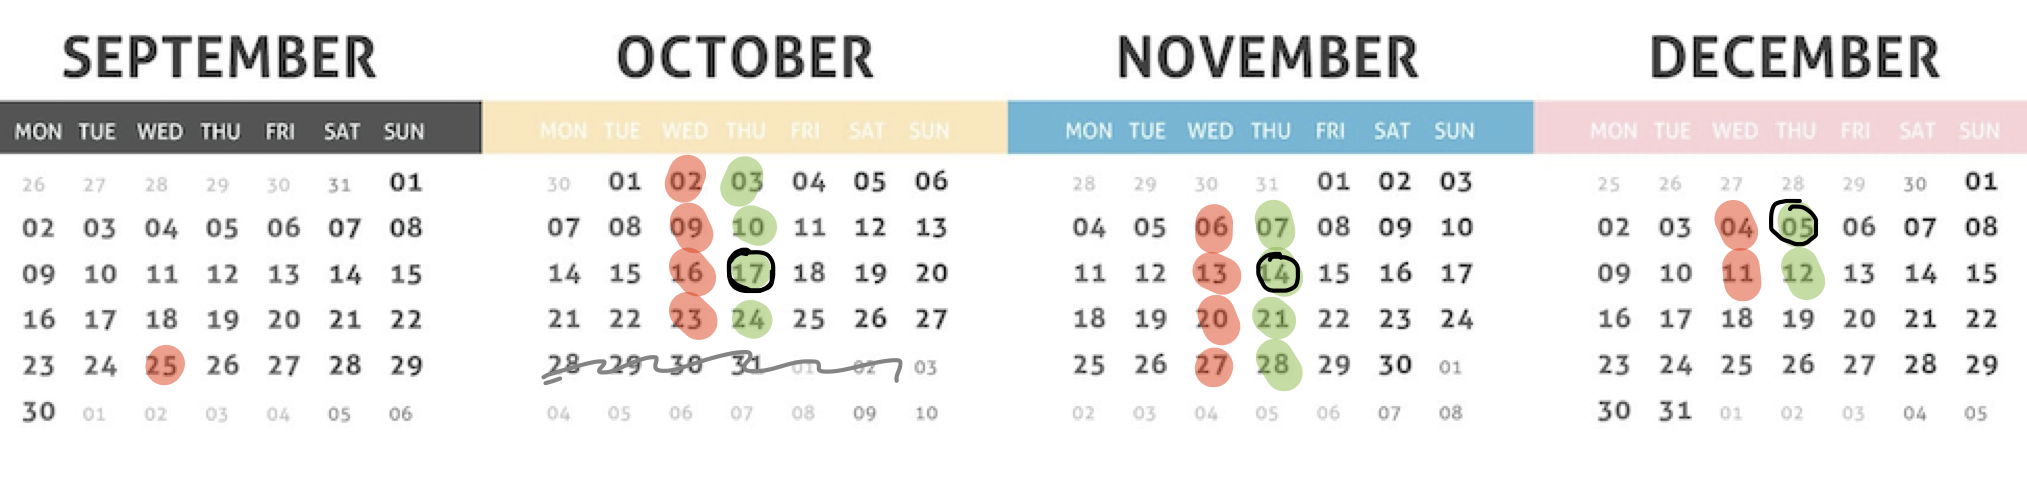
\includegraphics[width=0.95\textwidth]{./images/year_specific/phys201_calendar_201920_v1.png}\\
%   \end{center}
%
% \begin{itemize}
%   \item red circles: 2-hr lecture slots
%   \item green circles: 2-hr workshop slots
%   \item highlighted green circles: assessed workshops (tentative, may change)
% \end{itemize}
%
% \end{frame}

%
%
%

\begin{frame}{Aims of the course}

\begin{itemize}
{\small
\item
To introduce the fundamental concepts and principles of electrostatics, magnetostatics,
electromagnetism and Maxwell's equations, and electromagnetic waves.
\item
To introduce differential vector analysis in the context of electromagnetism.
\item
To introduce circuit principles and analysis (EMF, Ohm's law, Kirchhoff's rules, RC and RLC circuits)
\item
To introduce the formulation of Maxwell's equations in the presence of dielectric and magnetic materials.
\item
To develop the ability of students to apply Maxwell's equations to simple problems involving dielectric and
magnetic materials.
\item
To develop the concepts of field theories in Physics using electromagnetism as an example.
\item
To introduce light as an electromagnetic wave.
}
\end{itemize}

\vspace{0.2cm}
\noindent\rule{2cm}{0.4pt}\\
{\it \scriptsize Source: PHYS 201 module page in ORBIT.}

\end{frame}

%
% Syllabus
%

\begin{frame}{Syllabus}

\begin{itemize}
{\small
\item
Electric charge, Coulomb’s law, Charge density
\item
Electric field, Principle of Superposition
\item
Electric flux, Gauss’ law (integral form)
\item
Mutual potential energy of point charges, electric potential
\item
Calculating the field from the potential (gradient)
\item
Circulation, charges on conductors
\item
Gauss’ law in differential form (divergence)
\item
Circulation law in differential form (curl)
\item
Poisson’s and Laplace’s laws and solutions
\item
Electric dipole
\item
Electrostatics and conductors, method of images
\item
Gauss’ and Stokes’ theorems
\item
EMF, potential difference, electric current, current density
\item
Resistance, Ohm’s law
\item
Circuits, Kirkhhoff’s rules
}
\end{itemize}

\end{frame}


\begin{frame}{Syllabus cont'd}

\begin{itemize}
{\small
\item
Capacitance, calculation of capacitance for simple cases, RC circuits
\item
Dielectrics, polarization, electric displacement field
\item
Capacitance in the presence of dielectrics, force on a dielectric
\item
Magnetism, magnetic field, Biot-Savart law
\item
Lorentz force, force between currents
\item
Charged particle motion in magnetic field, velocity filter
\item
Magnetic dipole field, Ampere’s law in integral and differential forms
\item
Maxwell’s equations in vacuum for steady conditions
\item
Vector potential
\item
Magnetic materials, magnetization, magnetic field strength
\item
Maxwell’s equations in the presence of materials for steady conditions
\item
Motion of conductors inside magnetic fields, Faraday’s and Lenz’s laws
\item
Time-varying fields, Maxwell’s equations for the most general case
\item
Derivation of electromagnetic waves from Maxwell’s equations, speed of light
\item
LCR circuits
}
\end{itemize}

\vspace{0.2cm}
\noindent\rule{2cm}{0.4pt}\\
{\it \scriptsize Source: PHYS 201 module page in ORBIT.}

\end{frame}

%
%
%

\begin{frame}{Our approach will be calculus based}

\begin{itemize}
{
      \item We will explore several {\bf interesting physics concepts}.
      \item Our approach will be calculus-based.
      % \begin{itemize}
      % {
      %    \item for an interesting alternative approach, see here:\\
      %               {\color{blue} \tt http://videolectures.net/mit802s02\_electricity\_magnetism/}
      % }
      % \end{itemize}
      \item The electromagnetic phenomena are described by a set of {\bf very beautiful
                mathematical equations ({\em Maxwell} equations)}.
}
\end{itemize}


\begin{columns}
  \begin{column}{0.45\textwidth}
   \begin{center}
     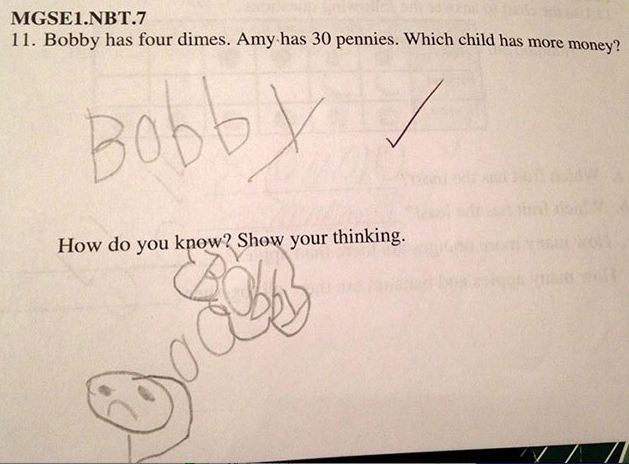
\includegraphics[width=0.80\textwidth]{./images/photos/bobby.png}\\
   \end{center}
  \end{column}
  \begin{column}{0.55\textwidth}
  {\small
         Mathematical dexterity necessary to
         \begin{itemize}
          { \small
                 \item sharpen your instinct
                 \item help you understand the connections between
                   different physics concepts
                  \item tackle practical problems
          }
         \end{itemize}
   }
  \end{column}
\end{columns}

\vspace{0.25cm}
{\bf Dust off your maths textbooks}! Its importance can not be overstated.\\

\end{frame}


%
%
%

\begin{frame}{Recommended textbooks - I}

Key texts:\\
\begin{itemize}
{\footnotesize
    \item D.J. Griffiths, `Introduction to Electrodynamics', Pearson, 2014\\
          {\scriptsize \color{blue} \url{https://library.liv.ac.uk/record=b4301805~S8}}
    \item D. Fleisch, `A Student's Guide to Maxwell's Equations', Cambridge, 2008\\
          {\scriptsize \color{blue} \url{https://library.liv.ac.uk/record=b2125525~S8}}\\
}
\end{itemize}

\end{frame}


\begin{frame}{Recommended textbooks - II}

Background reading:
\begin{itemize}
{\footnotesize
    \item The Feynman Lectures in Physics\\
          {\scriptsize \color{blue} \url{http://www.feynmanlectures.caltech.edu}}
    \item J.D. Jackson, Classical Electrodynamics, Wiley, 1998
          {\scriptsize \color{blue} \url{https://library.liv.ac.uk/record=b1783103~S8}}
    \item L.S. Grant and W.R. Phillips, `Electromagnetism', Wiley, 2013\\
          {\scriptsize \color{blue} \url{https://library.liv.ac.uk/record=b3130060~S8}}
    \item J. Walker, D. Halliday and R. Resnick, Fundamentals of Physics, Wiley, 2014\\
          {\scriptsize \color{blue} \url{https://library.liv.ac.uk/record=b2341872~S8}}
    \item D. Giancoli, Physics for Scientists and Engineers, Pearson, 2014\\
          {\scriptsize \color{blue} \url{https://library.liv.ac.uk/record=b2258154~S8}}
    \item D. Fleisch, `A Student's Guide to Vectors and Tensors', Cambridge, 2011\\
          {\scriptsize \color{blue} \url{https://library.liv.ac.uk/record=b2844947~S8}}
    \item G. Arfken, `Mathematical methods for physicists', Oxford, 2012\\
          {\scriptsize \color{blue} \url{https://library.liv.ac.uk/record=b2638836~S8}}
    \item J.C. Maxwell, Treatise on Electricity and Magnetism, 1873
          {\scriptsize \color{blue} \url{https://en.wikisource.org/wiki/A_Treatise_on_Electricity_and_Magnetism}}\\
}
\end{itemize}

\end{frame}


%
%
%

\begin{frame}{Slides / Handouts}

There are 4 types of slides:
{\color{darkpowderblue} Blue}, {\color{dBG1} Red},
{\color{eBG1} Orange}, and {\color{pBG1} Green}.

\begin{columns}
  \begin{column}{0.50\textwidth}
   \begin{center}
     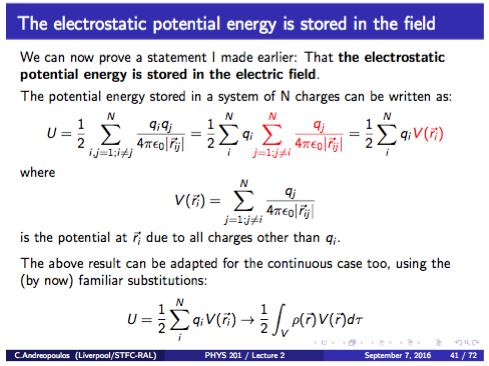
\includegraphics[width=0.7\textwidth]{./images/example_slides/main.png}\\
   \end{center}
  \end{column}
  \begin{column}{0.50\textwidth}
   \begin{center}
     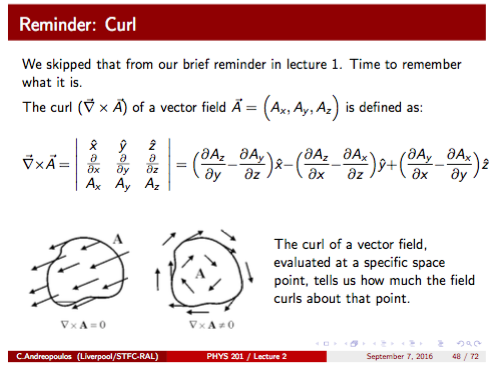
\includegraphics[width=0.7\textwidth]{./images/example_slides/reminder.png}\\
   \end{center}
  \end{column}
\end{columns}

\begin{columns}
  \begin{column}{0.50\textwidth}
   \begin{center}
     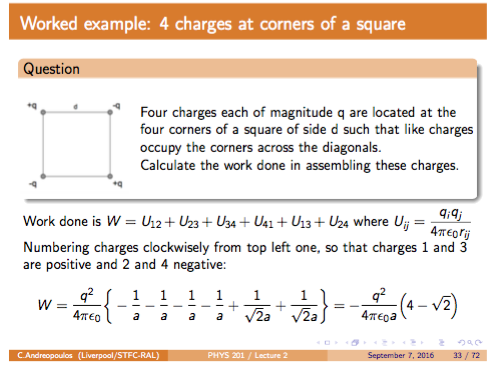
\includegraphics[width=0.7\textwidth]{./images/example_slides/worked_example.png}\\
   \end{center}
  \end{column}
  \begin{column}{0.50\textwidth}
   \begin{center}
     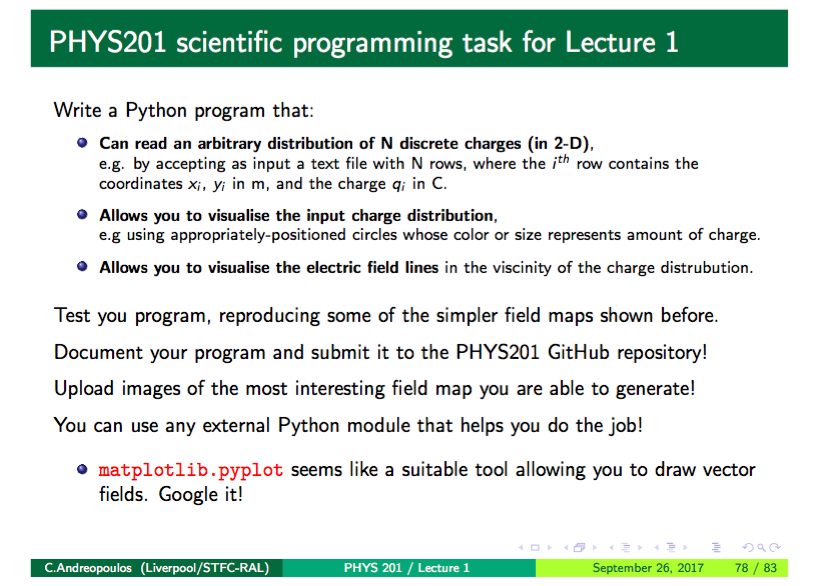
\includegraphics[width=0.7\textwidth]{./images/example_slides/python.png}\\
   \end{center}
  \end{column}
\end{columns}

\end{frame}


%
%
%

\begin{frame}{"Blue slides"}

\begin{columns}
  \begin{column}{0.30\textwidth}
   \begin{center}
        The main body of each PHYS201 lecture.\\
   \end{center}
  \end{column}
  \begin{column}{0.70\textwidth}
   \begin{center}
     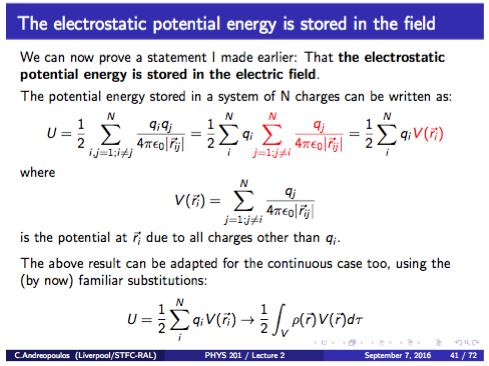
\includegraphics[width=0.99\textwidth]{./images/example_slides/main.png}\\
   \end{center}
  \end{column}
\end{columns}

\vspace{0.2cm}

\begin{center}
 {\bf Please check Canvas regularly for corrections and updates}.\\
\end{center}

\end{frame}

%
%
%

\begin{frame}{"Red slides"}

\begin{columns}
  \begin{column}{0.30\textwidth}
   \begin{center}
      Things you should already know / {\bf reminders}.\\
      \vspace{0.2cm}
      This material is here for easy reference!
      Typically, I will skip most of these slides during the lecture.\\
      \vspace{0.2cm}
      Please study the reminders in advance of each lecture.\\
   \end{center}
  \end{column}
  \begin{column}{0.70\textwidth}
   \begin{center}
     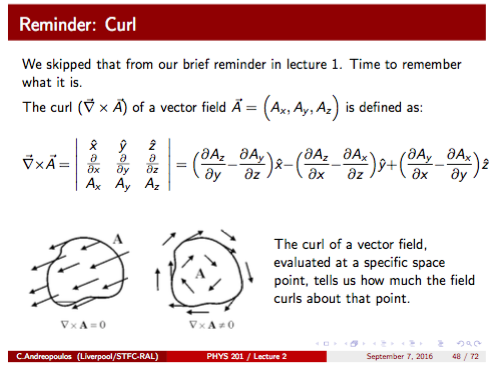
\includegraphics[width=0.99\textwidth]{./images/example_slides/reminder.png}\\
   \end{center}
  \end{column}
\end{columns}

\vspace{0.2cm}

\begin{center}
 {\bf Please check Canvas regularly for corrections and updates}.\\
\end{center}

\end{frame}


%
%
%


\begin{frame}{"Orange slides"}

\begin{columns}
  \begin{column}{0.30\textwidth}
   \begin{center}
      Questions and worked examples.\\
      \vspace{0.2cm}
      Will study as many as we have time for.
      More may be added in the digital version to address specific class needs.\\
   \end{center}
  \end{column}
  \begin{column}{0.70\textwidth}
   \begin{center}
     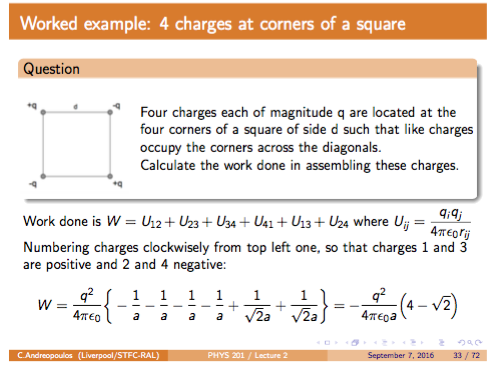
\includegraphics[width=0.99\textwidth]{./images/example_slides/worked_example.png}\\
   \end{center}
  \end{column}
\end{columns}

\vspace{0.2cm}

\begin{center}
 {\bf Please check Canvas regularly for corrections and updates}.\\
\end{center}

\end{frame}

%
%
%

\begin{frame}{"Green slides"}

\begin{columns}
  \begin{column}{0.52\textwidth}
     {\small
      Optional tasks (1/lecture) for which the analytical solution is too complex\\
      \vspace{0.2cm}
      Solve numerically, using C++/ROOT, Python or any other language (*)\\
      \vspace{0.2cm}
      Will be adding tasks, along with helpful hints, throughout the semester.\\
      \vspace{0.2cm}
      No marks awarded (optional tasks) but:
      \begin{itemize}
      {\scriptsize
        \item Improve your understanding of concepts!
        \item Gain experience in scientific computing!\\
      }
      \end{itemize}
     }
  \end{column}
  \begin{column}{0.48\textwidth}
   \begin{center}
     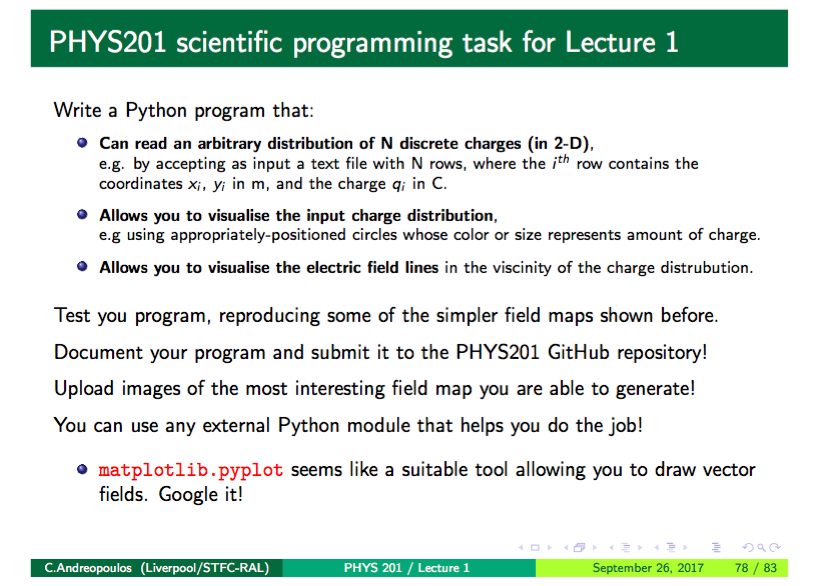
\includegraphics[width=0.99\textwidth]{./images/example_slides/python.png}\\
   \end{center}
  \end{column}
\end{columns}

\end{frame}

%
% -------------------------------------------------------------------------------
%

\begin{frame}{}
\begin{center}
{\Large Why is Electromagnetism one of your core modules?}
\end{center}
\end{frame}


\begin{frame}{Electromagnetism is one of the fundamental forces}

\underline{Main goal of physics}:
Study of the {\bf fundamental constituents of matter and of the forces between them}.\\
\vspace{0.2cm}

\begin{columns}
  \begin{column}{0.60\textwidth}
   \begin{center}
     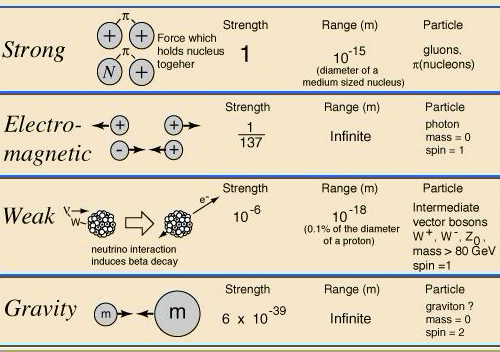
\includegraphics[width=0.98\textwidth]{./images/schematics/fundamental_forces.png}\\
   \end{center}
  \end{column}
  \begin{column}{0.40\textwidth}
    \begin{itemize}
    {\small
      \item Strong nuclear: keeps the atomic nucleus together
      \item {\color{magenta}Electromagnetism: the subject of this course.}
      \item Weak nuclear: responsible for nuclear $\beta$ decays
      \item Gravity: Pins you down on the Earth and rotates you around the Sun
    }
    \end{itemize}
  \end{column}
\end{columns}

\end{frame}

%
%
%

\begin{frame}{Electromagnetism}

\begin{columns}
     \begin{column}{0.33\textwidth}
       \begin{center}
          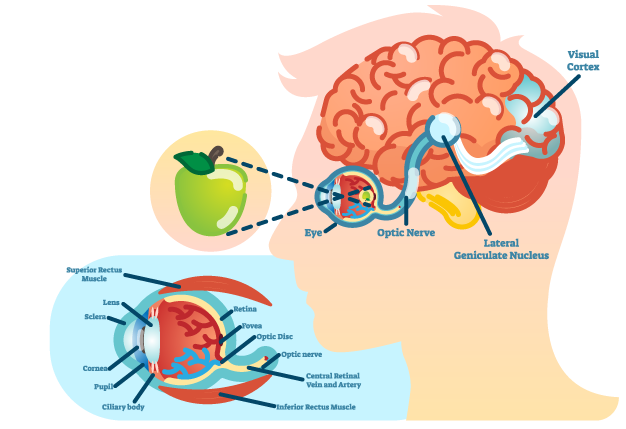
\includegraphics[width=0.90\textwidth]{./images/misc/vision_2.png}\\
       \end{center}
      \end{column}
      \begin{column}{0.33\textwidth}
        \begin{center}
          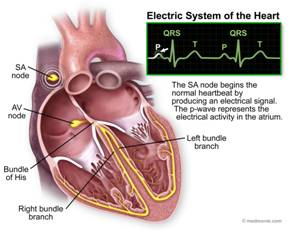
\includegraphics[width=0.90\textwidth]{./images/misc/electrical_system_heart.jpg}\\
        \end{center}
      \end{column}
      \begin{column}{0.33\textwidth}
        \begin{center}
          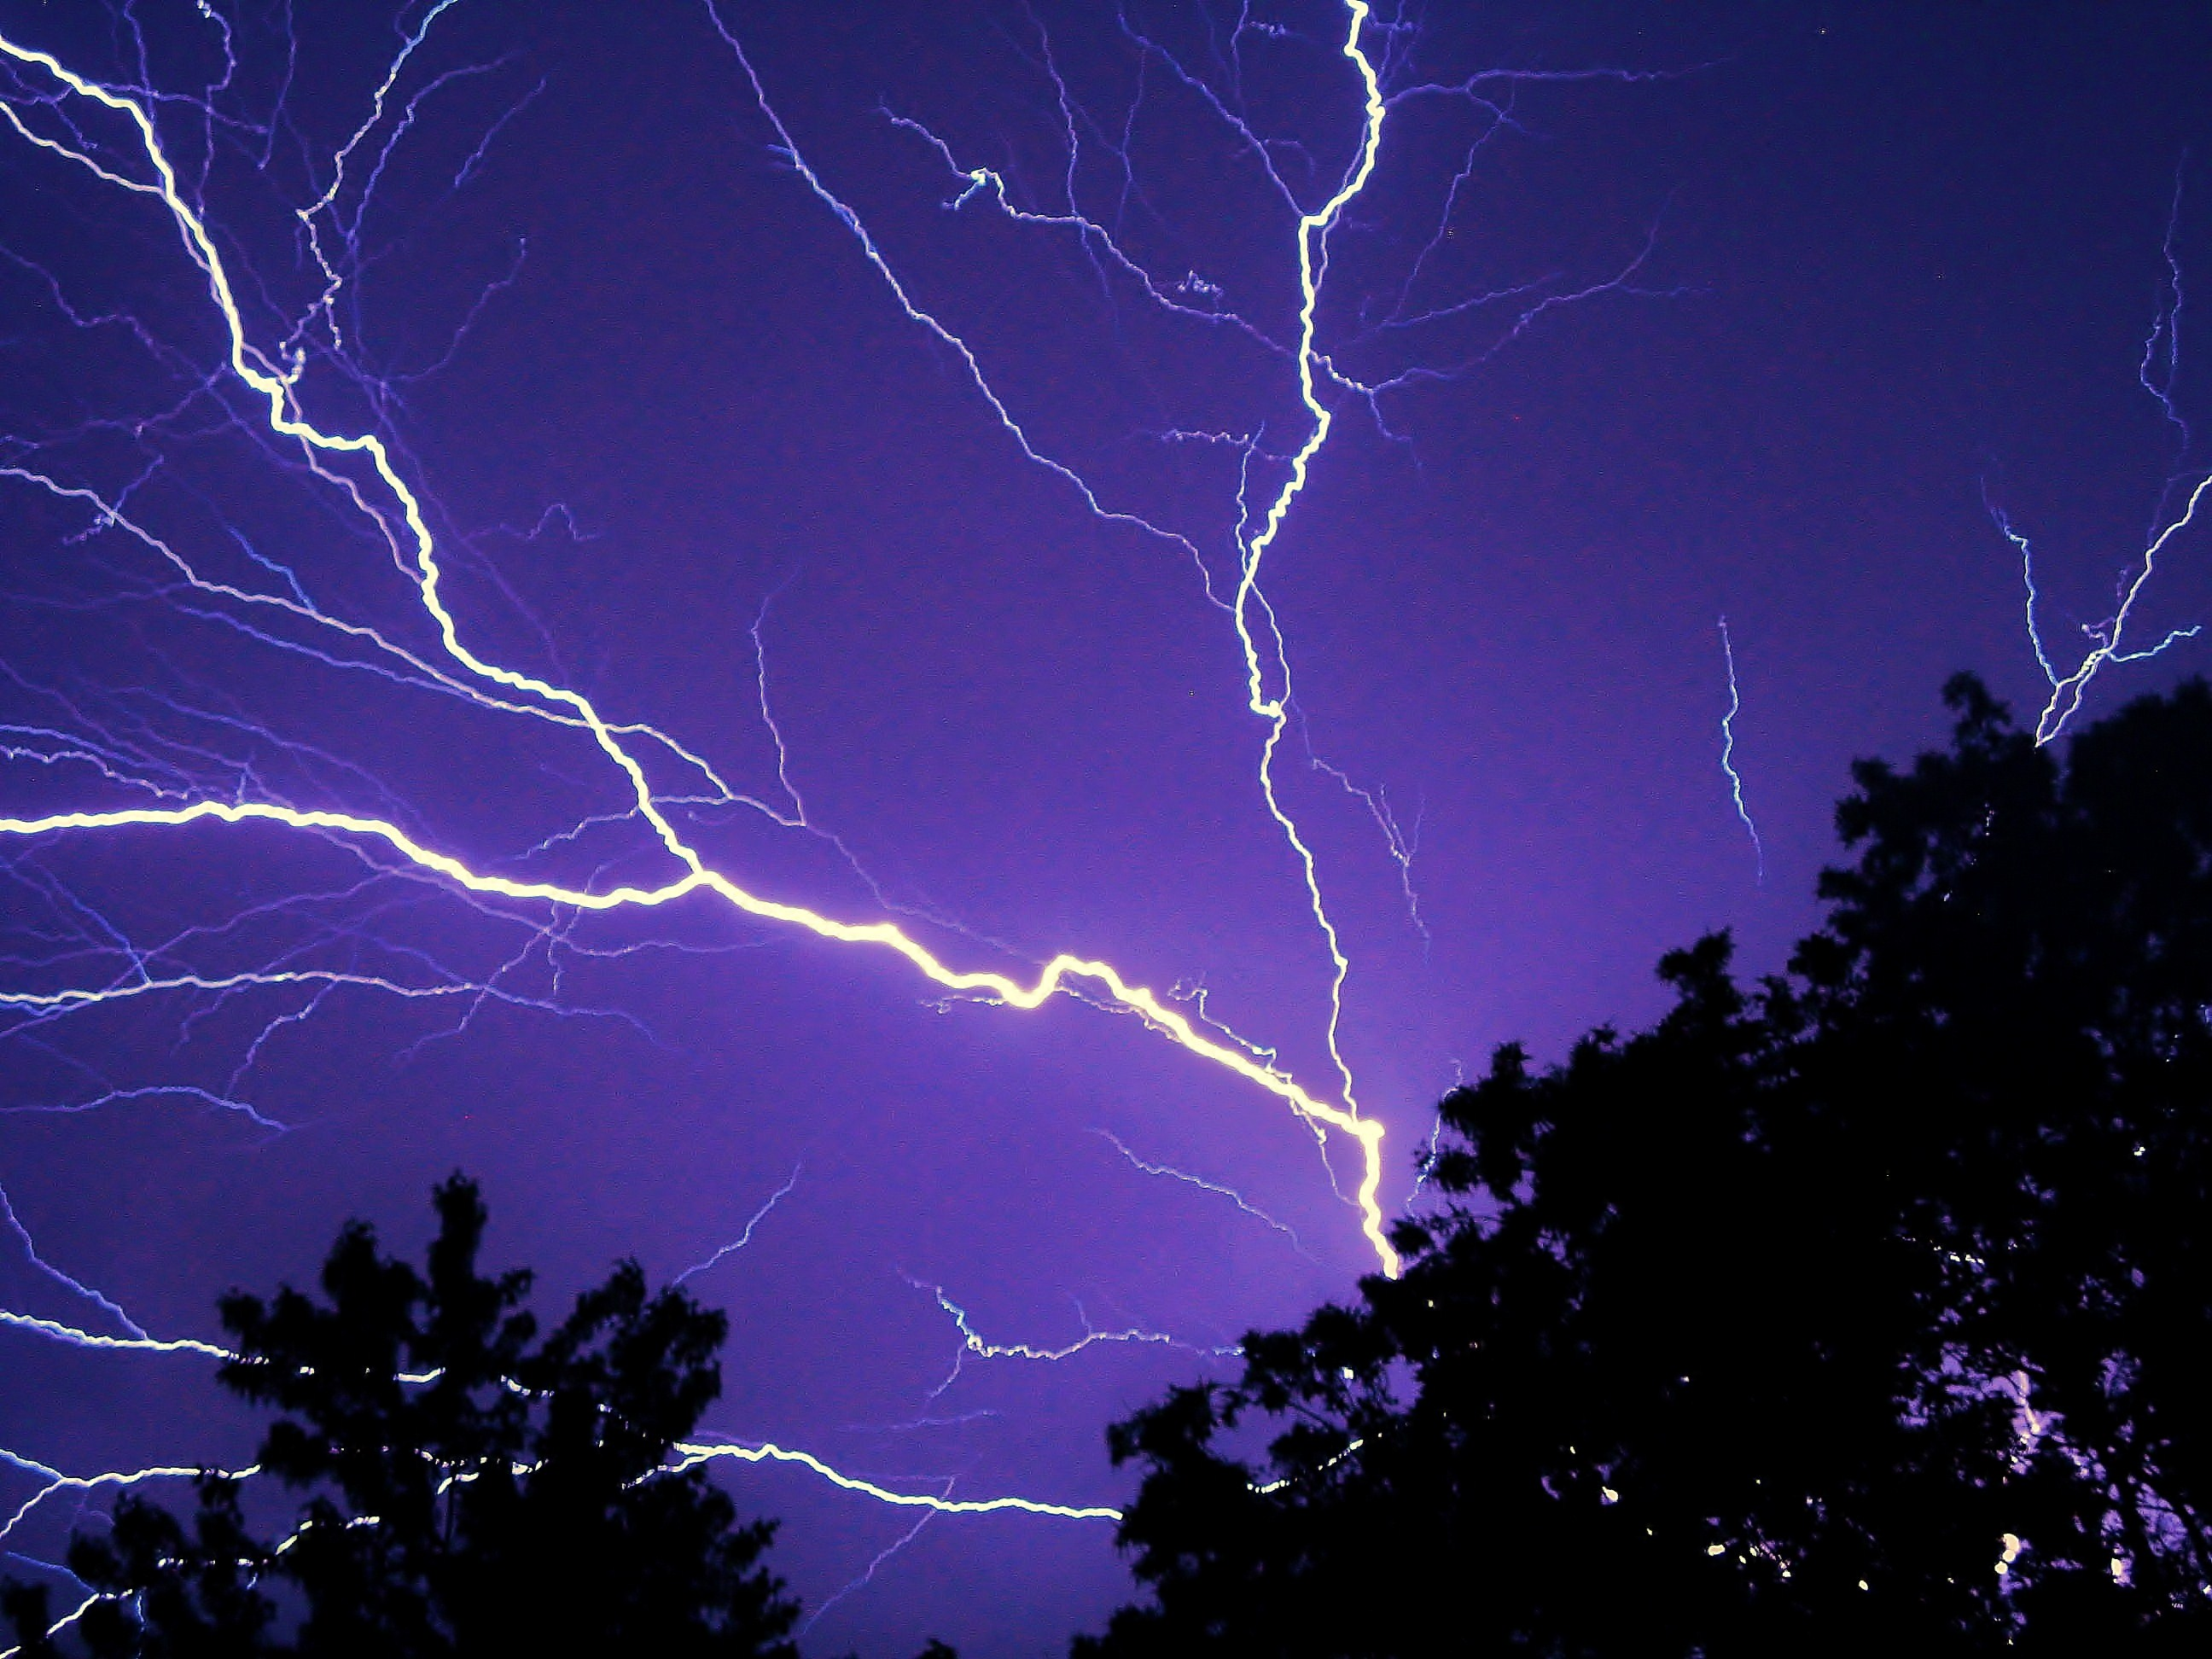
\includegraphics[width=0.90\textwidth]{./images/misc/lightning_1.jpg}\\
        \end{center}
      \end{column}
\end{columns}


\begin{center}
{\large
Electromagnetism {\bf underpins life, shapes our environment and our perception of it,
and is at the heart of technological innovations.}\\
}
\end{center}

\begin{columns}
     \begin{column}{0.25\textwidth}
       \begin{center}
          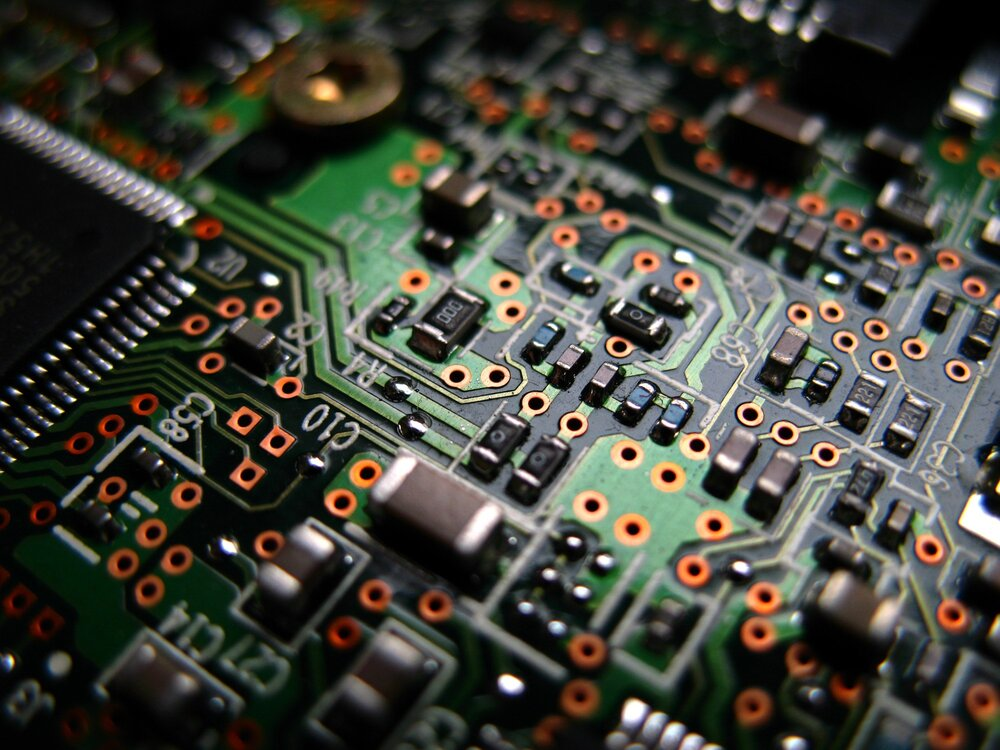
\includegraphics[width=0.99\textwidth]{./images/misc/circuit_1.jpg}\\
       \end{center}
      \end{column}
      \begin{column}{0.45\textwidth}
        \begin{center}
          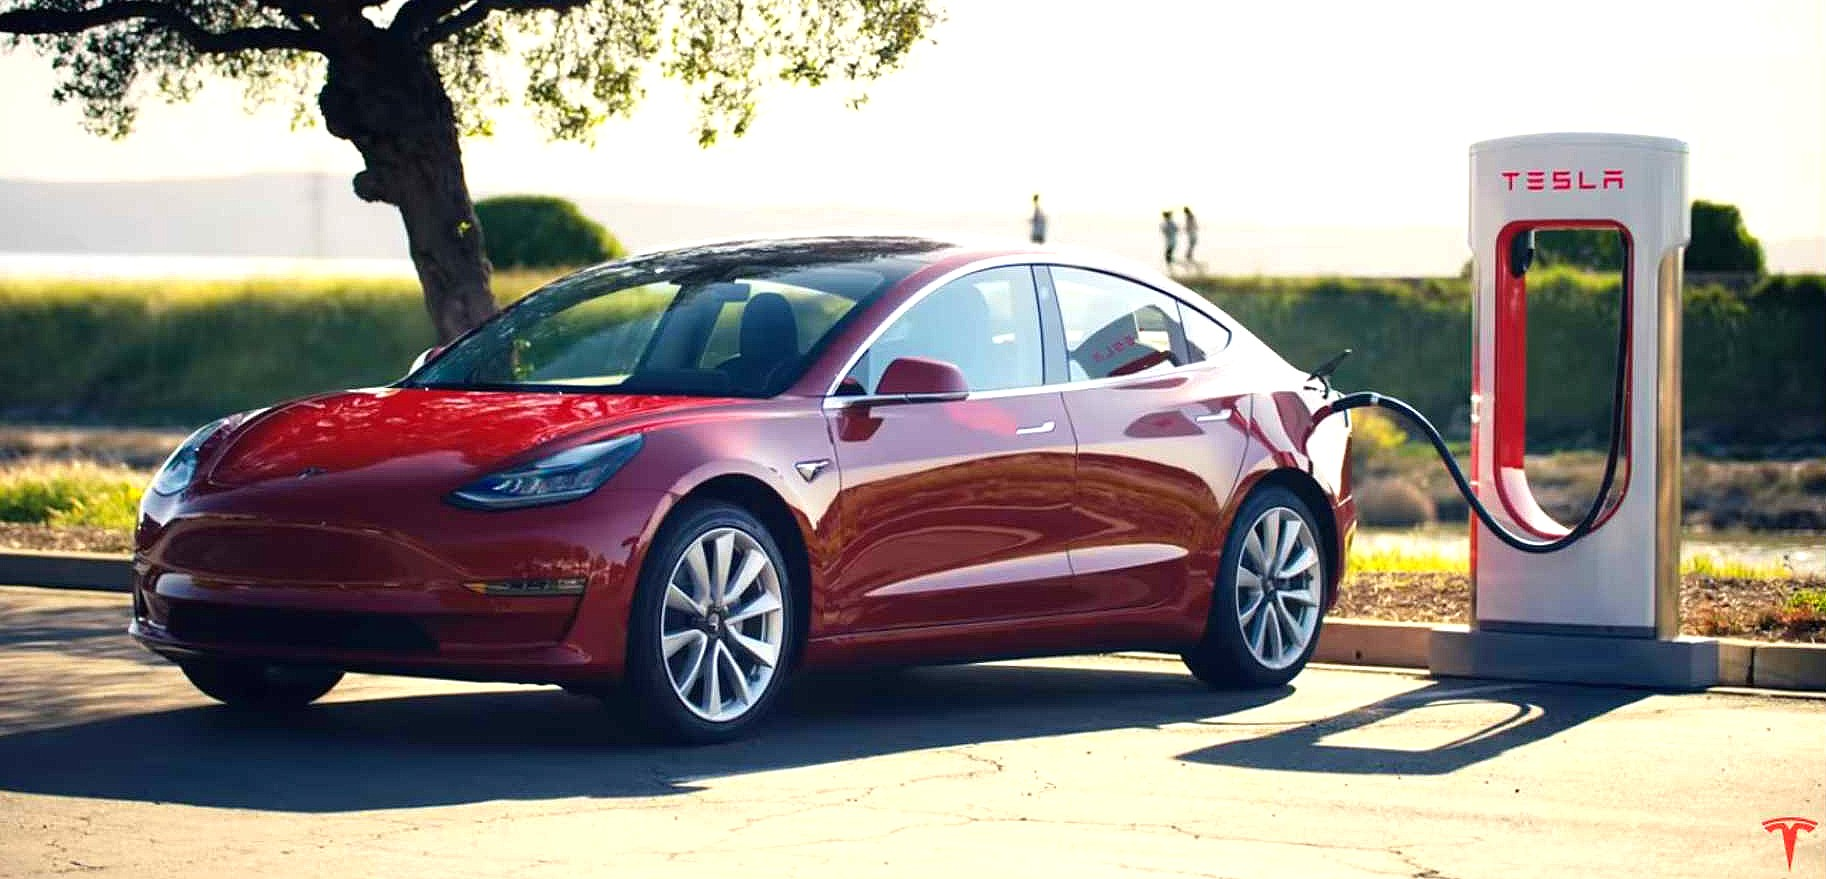
\includegraphics[width=0.90\textwidth]{./images/misc/tesla_1.jpg}\\
        \end{center}
      \end{column}
      \begin{column}{0.30\textwidth}
        \begin{center}
          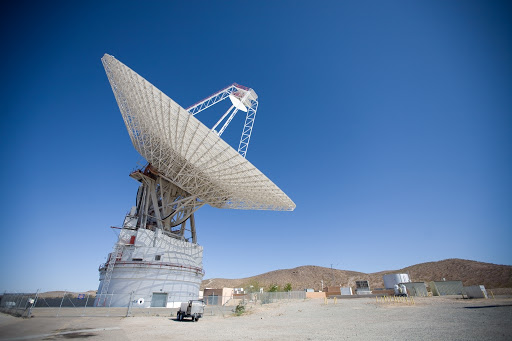
\includegraphics[width=0.92\textwidth]{./images/misc/radio_telescope_1.jpg}\\
        \end{center}
      \end{column}
\end{columns}

\end{frame}

%
%
%

\begin{frame}{Electromagnetism underpins life / chemistry}

  {\scriptsize
   You see me because {\bf light (an electromagnetic wave)} was scattered off me
   and interacted with photo-sensitive tissue in the retina of your eyes.
   This tissue generates {\bf electric signals} that travel to your
   brain via the optic nerve.
   In the visual cortex, through the electrical activity of many layers of neurons,
   your brain processes the input image.
  }

   \begin{center}
     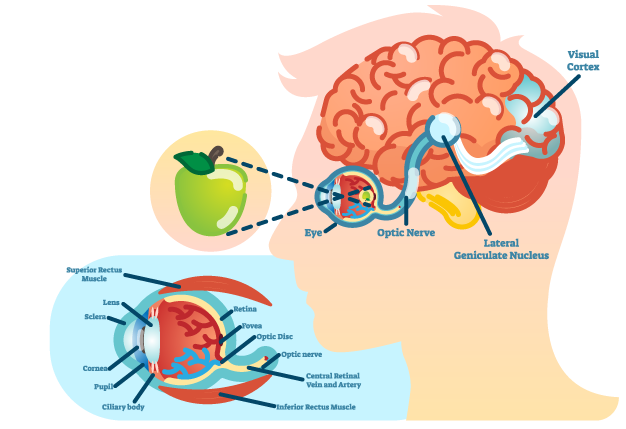
\includegraphics[width=0.70\textwidth]{./images/misc/vision_2.png}\\
   \end{center}

\end{frame}


\begin{frame}{Electromagnetism underpins life / chemistry}

  {\scriptsize
  The contraction of the muscles in your heart caused by
  {\bf electrical impulses} from the sinoatrial node.
  }

  \begin{center}
     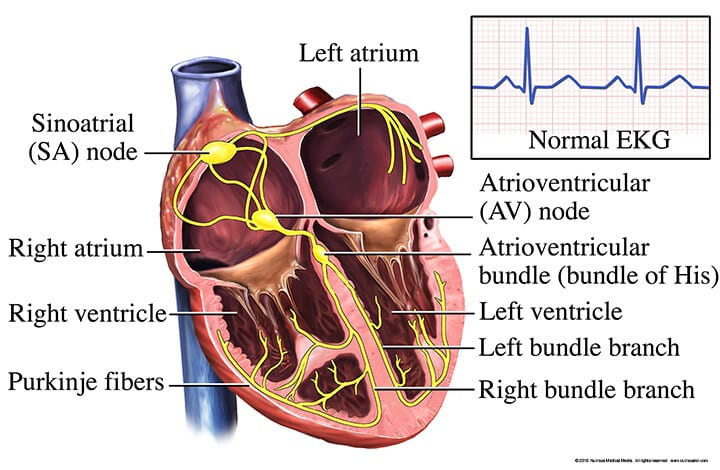
\includegraphics[width=0.75\textwidth]{./images/misc/electrical_system_heart_2.jpg}\\
  \end{center}

\end{frame}

%
%
%

\begin{frame}{Shapes our environment and our perception of it}

\begin{columns}
  \begin{column}{0.50\textwidth}
    {\scriptsize
     The feel of touching your desk, is the
     the {\bf electromagnetic repulsion between the electron clouds}
     in your hand and in your desk.\\
    }
    \begin{center}
     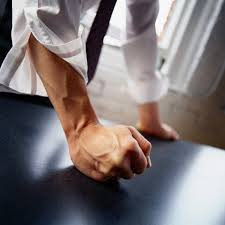
\includegraphics[width=0.80\textwidth]{./images/misc/hit_hand_on_desk.jpg}\\
    \end{center}
    \vspace{1.2cm}
  \end{column}
  \begin{column}{0.50\textwidth}
    {\scriptsize
      Vision/colour.\\
    }
    \begin{center}
     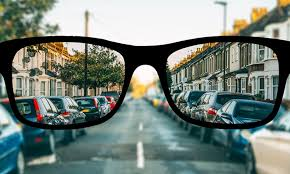
\includegraphics[width=0.60\textwidth]{./images/misc/vision_0.jpg}\\
    \end{center}
    {\scriptsize
      Chemical bonds arise from electric attraction between oppositely charged ions,
      or through the sharing of electric charges (electrons).\\
    }
    \begin{center}
     
\includegraphics[width=0.60\textwidth]{./images/misc/bonds.png}\\
    \end{center}

  \end{column}
\end{columns}

\end{frame}

%
%
%

\begin{frame}{Is at the heart of technological innovations}

  \begin{center}
    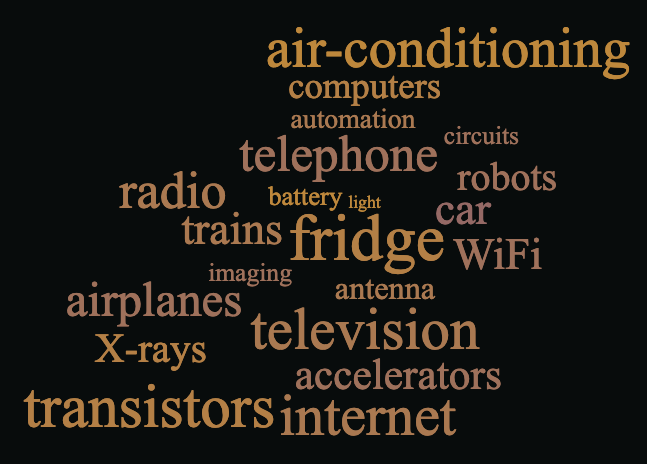
\includegraphics[width=0.80\textwidth]{./images/misc/word_cloud_apps.png}\\
  \end{center}

\end{frame}

%
%
%

\begin{frame}{Electric and magnetic forces known from ancient times}

\begin{columns}
    \begin{column}{0.90\textwidth}
    {\small
      Thales ($\sim$625-545 BC), a Greek Philosopher from Miletus (Asia Minor)
      has recorded observations of the properties of
      {\bf amber} and {\bf lodestones}.
    }
    \end{column}
    \begin{column}{0.10\textwidth}
      \begin{center}
         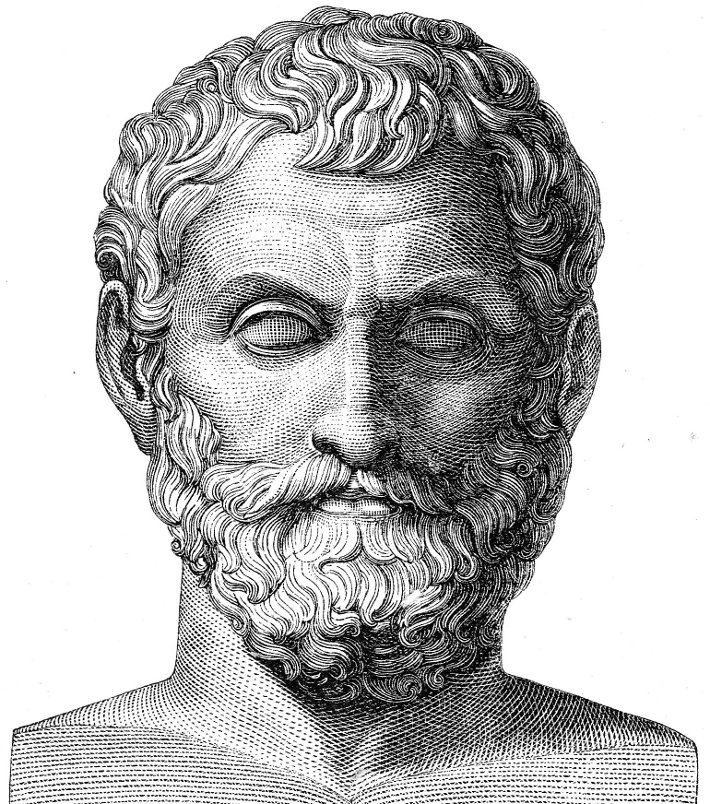
\includegraphics[width=0.90\textwidth]{./images/people/thales.jpg}\\
      \end{center}
    \end{column}
\end{columns}

\vspace{0.1cm}

\begin{columns}
  \begin{column}{0.20\textwidth}
   \begin{center}
      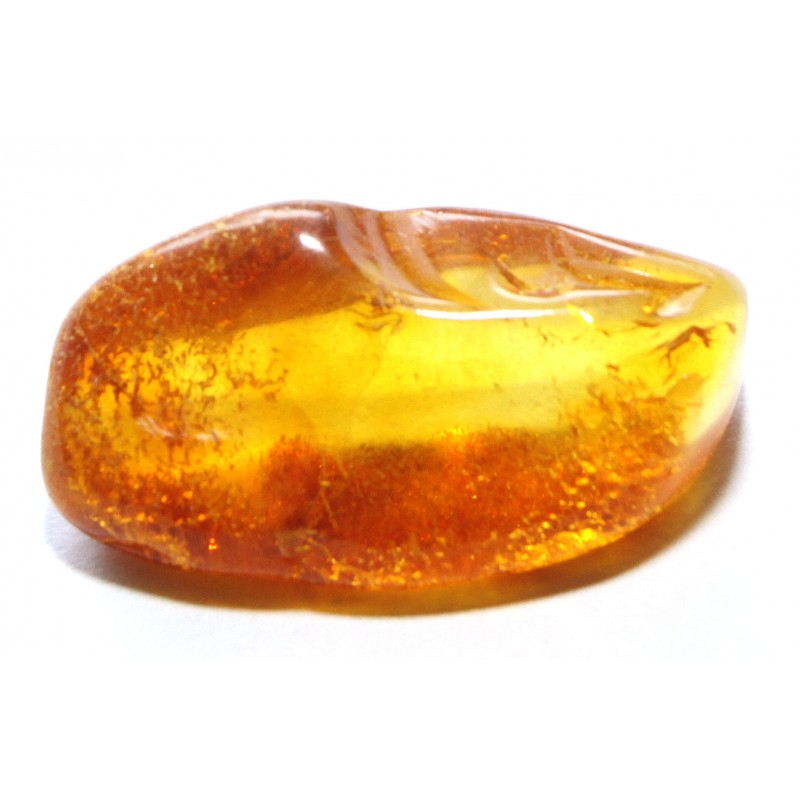
\includegraphics[width=0.95\textwidth]{./images/photos/amber_stone_1.jpg}\\
   \end{center}
  \end{column}
  \begin{column}{0.80\textwidth}
   \begin{itemize}
   {\small
    \item {\bf Amber}: a yellow-orange-brown fossilised tree resin
     \begin{itemize}
     {\scriptsize
        \item Amber is known as {\em `electron'} in Greek, the name given to first
              charged particle discovered and the origin of the term {\em electricity}.
     }
     \end{itemize}
     \item When rubbed with fur, amber could attract small bodies like small pieces of straw.
   }
   \end{itemize}
  \end{column}
\end{columns}

\vspace{0.2cm}

\begin{columns}
  \begin{column}{0.20\textwidth}
   \begin{center}
      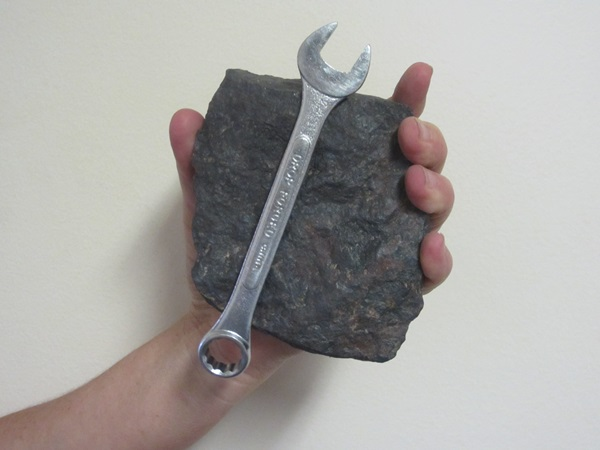
\includegraphics[width=0.90\textwidth]{./images/photos/lodestone_1.jpg}\\
   \end{center}
  \end{column}
  \begin{column}{0.80\textwidth}
   \begin{itemize}
    {\small
     \item {\bf Lodestone}: naturally magnetised piece of the mineral magnetite
     \begin{itemize}
     {\scriptsize
       \item Lodestones were first found in the Greek colony of {\em Magnesia},
             in what is now Asia minor, hence the term {\em magnetism}.
     }
     \end{itemize}
     \item Lodestone are attracted to iron and other lodestones.
    }
    \end{itemize}
  \end{column}
\end{columns}

\end{frame}


%
%
%

\begin{frame}{No further advance till the early modern period}

{\bf Electric and magnetic forces had an impact on early thinking}.\\
\begin{itemize}
   \item Electricity and magnetism perplexed Thales: How can an (inanimate) object attract other objects?
   \item This led him to believe that amber and lodestone may be alive?
     \begin{itemize}
        \item And then, perhaps, everything is living.\\
     \end{itemize}
\end{itemize}

\vspace{0.3cm}

There were some early applications
\begin{itemize}
   \item Magnetic compass (Chinese, 12th century AD; others)
\end{itemize}

\vspace{0.3cm}

But no further advance in understanding till the early modern period.
\begin{itemize}
    \item William Gilbert (1540-1603)
\end{itemize}

\end{frame}

%
%
%

\begin{frame}{Evolution of electromagnetic theory and applications}

\begin{itemize}

   \item The subject as we know it was {\bf developed in less than a century}
   \begin{itemize}
      \item $\sim$1785: Coulomb publishes his law
      \item $\sim$1864: Maxwell publishes his famous theory
        \begin{itemize}
            \item unity of electric and magnetic phenomena and understanding of light
        \end{itemize}
   \end{itemize}

   \item Several applications followed the development of the theory
   \begin{itemize}
     \item 1880: first wired-up house
     \item 1891: electric fan
     \item 1901: vacuum cleaner
     \item 1909: washing machine and iron
     \item 1918: refrigerator and dishwasher
     \item ...
   \end{itemize}
\end{itemize}

\begin{center}
  {\bf Try to imagine your life without electricity}!
\end{center}

\end{frame}

%
%
%

\begin{frame}{Electromagnetism in modern physics}

It is a wonderful example of a {\bf {\em covariant} theory}
\begin{itemize}
  \item The {\bf Special theory of relativity} had its origins in Classical Electrodynamics
\end{itemize}

\vspace{0.2cm}

Classical Electrodynamics coupled with Quantum Mechanics gives rise to {\bf Quantum Electrodynamics (QED)}
\begin{itemize}
  \item Experimentally tested to 1 in $10^{11}$ parts
  \begin{itemize}
     \item 1 in $10^{11}$: Like predicting the distance from New York to Los Angeles to about half the thickness of usual printer paper...
  \end{itemize}
  \item {\bf One of the most successful theories} ever built, and the most precisely tested one in the history of science.
  \item {\bf A prototype for other Quantum Field Theories}
\end{itemize}

\end{frame}
